\documentclass[twoside]{book}

% Packages required by doxygen
\usepackage{fixltx2e}
\usepackage{calc}
\usepackage{doxygen}
\usepackage[export]{adjustbox} % also loads graphicx
\usepackage{graphicx}
\usepackage[utf8]{inputenc}
\usepackage{makeidx}
\usepackage{multicol}
\usepackage{multirow}
\PassOptionsToPackage{warn}{textcomp}
\usepackage{textcomp}
\usepackage[nointegrals]{wasysym}
\usepackage[table]{xcolor}

% Font selection
\usepackage[T1]{fontenc}
\usepackage[scaled=.90]{helvet}
\usepackage{courier}
\usepackage{amssymb}
\usepackage{sectsty}
\renewcommand{\familydefault}{\sfdefault}
\allsectionsfont{%
  \fontseries{bc}\selectfont%
  \color{darkgray}%
}
\renewcommand{\DoxyLabelFont}{%
  \fontseries{bc}\selectfont%
  \color{darkgray}%
}
\newcommand{\+}{\discretionary{\mbox{\scriptsize$\hookleftarrow$}}{}{}}

% Page & text layout
\usepackage{geometry}
\geometry{%
  a4paper,%
  top=2.5cm,%
  bottom=2.5cm,%
  left=2.5cm,%
  right=2.5cm%
}
\tolerance=750
\hfuzz=15pt
\hbadness=750
\setlength{\emergencystretch}{15pt}
\setlength{\parindent}{0cm}
\setlength{\parskip}{3ex plus 2ex minus 2ex}
\makeatletter
\renewcommand{\paragraph}{%
  \@startsection{paragraph}{4}{0ex}{-1.0ex}{1.0ex}{%
    \normalfont\normalsize\bfseries\SS@parafont%
  }%
}
\renewcommand{\subparagraph}{%
  \@startsection{subparagraph}{5}{0ex}{-1.0ex}{1.0ex}{%
    \normalfont\normalsize\bfseries\SS@subparafont%
  }%
}
\makeatother

% Headers & footers
\usepackage{fancyhdr}
\pagestyle{fancyplain}
\fancyhead[LE]{\fancyplain{}{\bfseries\thepage}}
\fancyhead[CE]{\fancyplain{}{}}
\fancyhead[RE]{\fancyplain{}{\bfseries\leftmark}}
\fancyhead[LO]{\fancyplain{}{\bfseries\rightmark}}
\fancyhead[CO]{\fancyplain{}{}}
\fancyhead[RO]{\fancyplain{}{\bfseries\thepage}}
\fancyfoot[LE]{\fancyplain{}{}}
\fancyfoot[CE]{\fancyplain{}{}}
\fancyfoot[RE]{\fancyplain{}{\bfseries\scriptsize Generated by Doxygen }}
\fancyfoot[LO]{\fancyplain{}{\bfseries\scriptsize Generated by Doxygen }}
\fancyfoot[CO]{\fancyplain{}{}}
\fancyfoot[RO]{\fancyplain{}{}}
\renewcommand{\footrulewidth}{0.4pt}
\renewcommand{\chaptermark}[1]{%
  \markboth{#1}{}%
}
\renewcommand{\sectionmark}[1]{%
  \markright{\thesection\ #1}%
}

% Indices & bibliography
\usepackage{natbib}
\usepackage[titles]{tocloft}
\setcounter{tocdepth}{3}
\setcounter{secnumdepth}{5}
\makeindex

% Hyperlinks (required, but should be loaded last)
\usepackage{ifpdf}
\ifpdf
  \usepackage[pdftex,pagebackref=true]{hyperref}
\else
  \usepackage[ps2pdf,pagebackref=true]{hyperref}
\fi
\hypersetup{%
  colorlinks=true,%
  linkcolor=blue,%
  citecolor=blue,%
  unicode%
}

% Custom commands
\newcommand{\clearemptydoublepage}{%
  \newpage{\pagestyle{empty}\cleardoublepage}%
}

\usepackage{caption}
\captionsetup{labelsep=space,justification=centering,font={bf},singlelinecheck=off,skip=4pt,position=top}

%===== C O N T E N T S =====

\begin{document}

% Titlepage & ToC
\hypersetup{pageanchor=false,
             bookmarksnumbered=true,
             pdfencoding=unicode
            }
\pagenumbering{alph}
\begin{titlepage}
\vspace*{7cm}
\begin{center}%
{\Large \textquotesingle{}Figure\textquotesingle{} }\\
\vspace*{1cm}
{\large Generated by Doxygen 1.8.13}\\
\end{center}
\end{titlepage}
\clearemptydoublepage
\pagenumbering{roman}
\tableofcontents
\clearemptydoublepage
\pagenumbering{arabic}
\hypersetup{pageanchor=true}

%--- Begin generated contents ---
\chapter{Hierarchical Index}
\section{Class Hierarchy}
This inheritance list is sorted roughly, but not completely, alphabetically\+:\begin{DoxyCompactList}
\item \contentsline{section}{Figure}{\pageref{classFigure}}{}
\begin{DoxyCompactList}
\item \contentsline{section}{Disque}{\pageref{classDisque}}{}
\item \contentsline{section}{Rectangle}{\pageref{classRectangle}}{}
\item \contentsline{section}{Triangle}{\pageref{classTriangle}}{}
\end{DoxyCompactList}
\end{DoxyCompactList}

\chapter{Class Index}
\section{Class List}
Here are the classes, structs, unions and interfaces with brief descriptions\+:\begin{DoxyCompactList}
\item\contentsline{section}{\hyperlink{classDisque}{Disque} }{\pageref{classDisque}}{}
\item\contentsline{section}{\hyperlink{classFigure}{Figure} }{\pageref{classFigure}}{}
\item\contentsline{section}{\hyperlink{classRectangle}{Rectangle} }{\pageref{classRectangle}}{}
\item\contentsline{section}{\hyperlink{classTriangle}{Triangle} }{\pageref{classTriangle}}{}
\end{DoxyCompactList}

\chapter{Class Documentation}
\hypertarget{classDisque}{}\section{Disque Class Reference}
\label{classDisque}\index{Disque@{Disque}}


Inheritance diagram for Disque\+:
\nopagebreak
\begin{figure}[H]
\begin{center}
\leavevmode
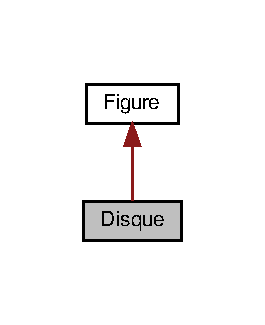
\includegraphics[width=127pt]{classDisque__inherit__graph}
\end{center}
\end{figure}


Collaboration diagram for Disque\+:
\nopagebreak
\begin{figure}[H]
\begin{center}
\leavevmode
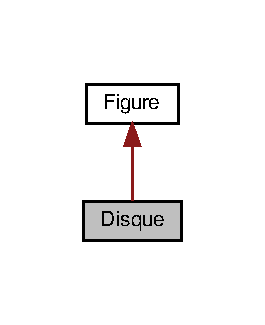
\includegraphics[width=127pt]{classDisque__coll__graph}
\end{center}
\end{figure}
\subsection*{Public Member Functions}
\begin{DoxyCompactItemize}
\item 
\mbox{\Hypertarget{classDisque_a5c2ef8ccfa24309f18acaa6b21b1d7b3}\label{classDisque_a5c2ef8ccfa24309f18acaa6b21b1d7b3}} 
void {\bfseries set\+Rayon} ()
\item 
\mbox{\Hypertarget{classDisque_a7c0cc5813b36ab93977fb0f66aa5e470}\label{classDisque_a7c0cc5813b36ab93977fb0f66aa5e470}} 
float {\bfseries perimetre} ()
\item 
\mbox{\Hypertarget{classDisque_aacd8d27b8d47bea0cb749dac208710c8}\label{classDisque_aacd8d27b8d47bea0cb749dac208710c8}} 
float {\bfseries surface} ()
\end{DoxyCompactItemize}


The documentation for this class was generated from the following files\+:\begin{DoxyCompactItemize}
\item 
/home/macron/cpp/figure/src/Disque.\+h\item 
/home/macron/cpp/figure/src/Disque.\+cpp\end{DoxyCompactItemize}

\hypertarget{classFigure}{}\section{Figure Class Reference}
\label{classFigure}\index{Figure@{Figure}}


Inheritance diagram for Figure\+:
\nopagebreak
\begin{figure}[H]
\begin{center}
\leavevmode
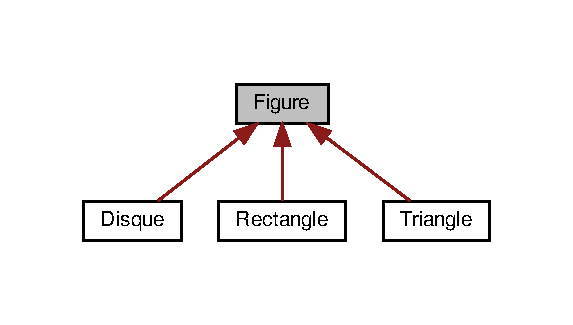
\includegraphics[width=275pt]{classFigure__inherit__graph}
\end{center}
\end{figure}
\subsection*{Protected Member Functions}
\begin{DoxyCompactItemize}
\item 
\mbox{\Hypertarget{classFigure_a82a6ec992970471c1e7ae9b7a66d9008}\label{classFigure_a82a6ec992970471c1e7ae9b7a66d9008}} 
float {\bfseries perimetre} ()
\item 
\mbox{\Hypertarget{classFigure_a4b0cc8fdc08b636ffbe71342dbd11af4}\label{classFigure_a4b0cc8fdc08b636ffbe71342dbd11af4}} 
float {\bfseries surface} ()
\end{DoxyCompactItemize}


The documentation for this class was generated from the following file\+:\begin{DoxyCompactItemize}
\item 
/home/macron/cpp/figure/src/Figure.\+h\end{DoxyCompactItemize}

\hypertarget{classRectangle}{}\section{Rectangle Class Reference}
\label{classRectangle}\index{Rectangle@{Rectangle}}


Inheritance diagram for Rectangle\+:
\nopagebreak
\begin{figure}[H]
\begin{center}
\leavevmode
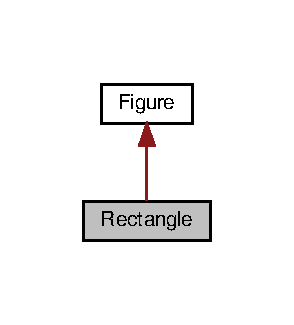
\includegraphics[width=141pt]{classRectangle__inherit__graph}
\end{center}
\end{figure}


Collaboration diagram for Rectangle\+:
\nopagebreak
\begin{figure}[H]
\begin{center}
\leavevmode
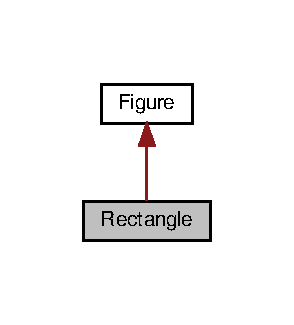
\includegraphics[width=141pt]{classRectangle__coll__graph}
\end{center}
\end{figure}
\subsection*{Public Member Functions}
\begin{DoxyCompactItemize}
\item 
\mbox{\Hypertarget{classRectangle_ac082860a64438de4b24929b2c3ec0d64}\label{classRectangle_ac082860a64438de4b24929b2c3ec0d64}} 
void {\bfseries set\+Longueur} ()
\item 
\mbox{\Hypertarget{classRectangle_af4d96a3a059d94ce90bdce7adc96471b}\label{classRectangle_af4d96a3a059d94ce90bdce7adc96471b}} 
void {\bfseries set\+Largeur} ()
\item 
\mbox{\Hypertarget{classRectangle_aabf428250df2d89c2c99e1692acde087}\label{classRectangle_aabf428250df2d89c2c99e1692acde087}} 
float {\bfseries perimetre} ()
\item 
\mbox{\Hypertarget{classRectangle_a388d3e127eb88cecf576fc861d938f5a}\label{classRectangle_a388d3e127eb88cecf576fc861d938f5a}} 
float {\bfseries surface} ()
\end{DoxyCompactItemize}


The documentation for this class was generated from the following files\+:\begin{DoxyCompactItemize}
\item 
/home/macron/cpp/figure/src/Rectangle.\+h\item 
/home/macron/cpp/figure/src/Rectangle.\+cpp\end{DoxyCompactItemize}

\hypertarget{classTriangle}{}\section{Triangle Class Reference}
\label{classTriangle}\index{Triangle@{Triangle}}


Inheritance diagram for Triangle\+:
\nopagebreak
\begin{figure}[H]
\begin{center}
\leavevmode
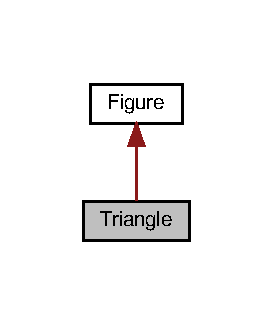
\includegraphics[width=131pt]{classTriangle__inherit__graph}
\end{center}
\end{figure}


Collaboration diagram for Triangle\+:
\nopagebreak
\begin{figure}[H]
\begin{center}
\leavevmode
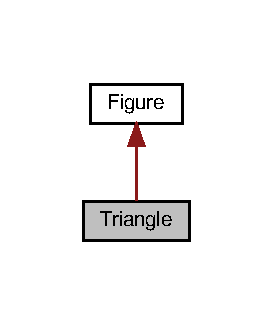
\includegraphics[width=131pt]{classTriangle__coll__graph}
\end{center}
\end{figure}
\subsection*{Public Member Functions}
\begin{DoxyCompactItemize}
\item 
\mbox{\Hypertarget{classTriangle_a7c7f471befc770547cc00677a42b7b72}\label{classTriangle_a7c7f471befc770547cc00677a42b7b72}} 
void {\bfseries set\+Base} ()
\item 
\mbox{\Hypertarget{classTriangle_ae84e07501830b6da3113ebc7c1a5ac8b}\label{classTriangle_ae84e07501830b6da3113ebc7c1a5ac8b}} 
void {\bfseries set\+Hauteur} ()
\item 
\mbox{\Hypertarget{classTriangle_a4ebfa1b94dbb6eb0eb1bc437cefad3a2}\label{classTriangle_a4ebfa1b94dbb6eb0eb1bc437cefad3a2}} 
float {\bfseries perimetre} ()
\item 
\mbox{\Hypertarget{classTriangle_adcc6c150141934d6d53db85bcca93958}\label{classTriangle_adcc6c150141934d6d53db85bcca93958}} 
float {\bfseries surface} ()
\end{DoxyCompactItemize}


The documentation for this class was generated from the following files\+:\begin{DoxyCompactItemize}
\item 
/home/macron/cpp/figure/src/Triangle.\+h\item 
/home/macron/cpp/figure/src/Triangle.\+cpp\end{DoxyCompactItemize}

%--- End generated contents ---

% Index
\backmatter
\newpage
\phantomsection
\clearemptydoublepage
\addcontentsline{toc}{chapter}{Index}
\printindex

\end{document}
